\documentclass{article}
\usepackage[utf8]{inputenc}
\usepackage{graphicx,epsf,ulem}
\usepackage{float}
\usepackage[margin=1.0in]{geometry}
\usepackage{textgreek}
\begin{document}
\title{2D Ising Model Simulation with Varying Adjacent Site Configurations}
\author{Yanall Boutros}
\date{\today}
\maketitle
\section*{I. Introduction}
\indent \indent The Ising model is a model which displays the termodynamic
properties of a ferromagnet by simulating the interactions of $N^2$  atoms
(or spin-sites) on an $N\times N$ grid. The simulation flips a random spin-site
by a factor of $-1$ and if the change in spin causes the energy change in the
system to follow the Boltzmann Distribution, then the model saves that change.

\indent The change in energy is proportional to the sum of the spin-states
adjacent to the test spin-site, typically the 2D ising model considers the 
spin sites $S_{i+1, j}$, $S_{i, j+1}$, $S_{i-1, j}$, and $S_{i, j-1}$ to 
be adjacent to a spin site $S_{i, j}$. In this experiment, different definitions
for adjacent spin-sites are implemented to observe how the physical properties
and structure of the lattice change.
\section*{II. Background and Theory}
\indent \indent The $2D$ Ising model contains some characteristics not present
in the $1D$ Ising model, such as phase transitions. These transitions can be
observed qualitatevly by watching how the structure of the model gradually 
decomposes, and quantitavely via notable inflection points in the energy $E$,
magnitization $M$, and specific heat $C_v$ vs $k_bT$ graphs.

\indent The initial energy of the state is determined by implementing a
checkerboard algorithm over the state, and is vectorized to improve effiency.
In the following function, $Roll(\vec{V}, n)$ is defined to rotate all elements 
in a vector $\vec{V}$ by $n$ indices, with end elements rotating to the front.
Therefore, the total energy of a state composed of $R$ row vectors and $C$ column
vectors, with transfer energy $J$, magnetic moment $\mu$,
in a magnetic field $B$ is given by
\begin{equation}
  E = -J\sum_0^R Roll(\vec{V_R}, 1) \cdot \vec{V_R} + \sum_0^R -\mu B\vec{V_R} \cdot
  \vec{I}
  -J\sum_0^C Roll(\vec{V_C}, 1) \cdot \vec{V_C} + \sum_0^C -\mu B\vec{V_C} \cdot \vec{I}
\end{equation}
Where $\vec{I}$ is the identity matrix.
$M$ is given simply by
\begin{equation}
  \sum_{i,j} S_{i,j}
\end{equation}
and $C_v$ is given by
\begin{equation}
  C_v = \frac{1}{N^2}
  \frac{\left\langle E\right\rangle^2 - \left\langle E^2\right\rangle}{k_BT^2}
\end{equation}
\indent The change in energy $\Delta E$ depends on how we define what is considered
adjacent spin-sites, and is detailed in \textbf{Section III}.
In matter, the shape of the electron orbitals influence what
are adjacent spin-sites. For example, if two sheets of a material are parallel in 
the $x-z$ plane, and have electron orbitals that extend in the $x-z$ plane, then
the two sheets do not interact and the interacting neighbors would only be along
the $x-z$ plane, but if the electron orbitals span the $x-y$ plane, then the two
sheets are able to interact. When the adjacent spin-sites of $S_{i,j}$ are defined
to include all 8 adjacent neighbors (including the diagonal elements) then we 
begin to see the structure of the material begin to resemble a maze like 
pattern, seemingly similar to bizmuth (although I am uncertain if bizmuth's
electron configuration matches this definition of adjaceny).
\section*{III. Implementation}
\indent \indent This simulation follows from the logic behind the Metropolis algorithm
and Monte Carlo methods. For each temperature $kt$ in the domain of all
temperatures $T$,  run the simulation for given values of $J$, $\mu$, and $B$.
Calculate the initial energy (as described above) and the initial magnetization.
Generate a list of random spin-site locations, the length of which is the number
of time steps to iterate for. In this simulation we chose 20 times the number of 
spin-sites. For each coordinate $co$ in our list, multiply the value of the
spin-site by $-1$. If the change in energy follows the Boltzmann's distribution,
we keep the change, and update our values of energy. The change in magnitization 
is also calculated. After the simulation runs for that value of $kt$, the energy
versus time is plotted, and other physical parameters are recorded. After the
simulation is done running for all valus of $kt$, the average equilibrium energy
vs $kT$, the average magnitzation vs $kT$ and the specific heat versus $kT$ are
plotted. Finally, an animation is rendered showing how the simulation changes from
our initial $kT$ to our final, for all time steps.

\indent $\Delta E$ depends on the definition of what is an adjacent spin-site. 
Our trials included three main definitions for adjacent sites: grid-adjacent,
all-adjacent, and diag-adjacent. grid-adjacent is defined above in the 
\textbf{Introduction} and is the standard used in the 2D Ising model. All-adjacent
is defined to include the diagonal sites as well, and diag-adjacent is only 
the diagonal components.
\section*{IV. Results}
\indent \indent Figures 1 - 12 are provided below, and contain for each different site adjacency type
the energy vs time graphs at $kT = 1$, the average energy vs $kT$, the average 
magnitzation vs $kT$, and the specific heat vs $kT$. The source code for this 
project, as well as pdfs containing the energy vs time graphs for each $kT$, as 
well as animations displaying the change in our state configuration, are all
available in the zipped filesystem this report is contained in.
\subsection*{Grid-adjacent}
\begin{figure}[H]
  \caption{\textit{(left)} Plot of Energy vs Time for $kT = 1$}
  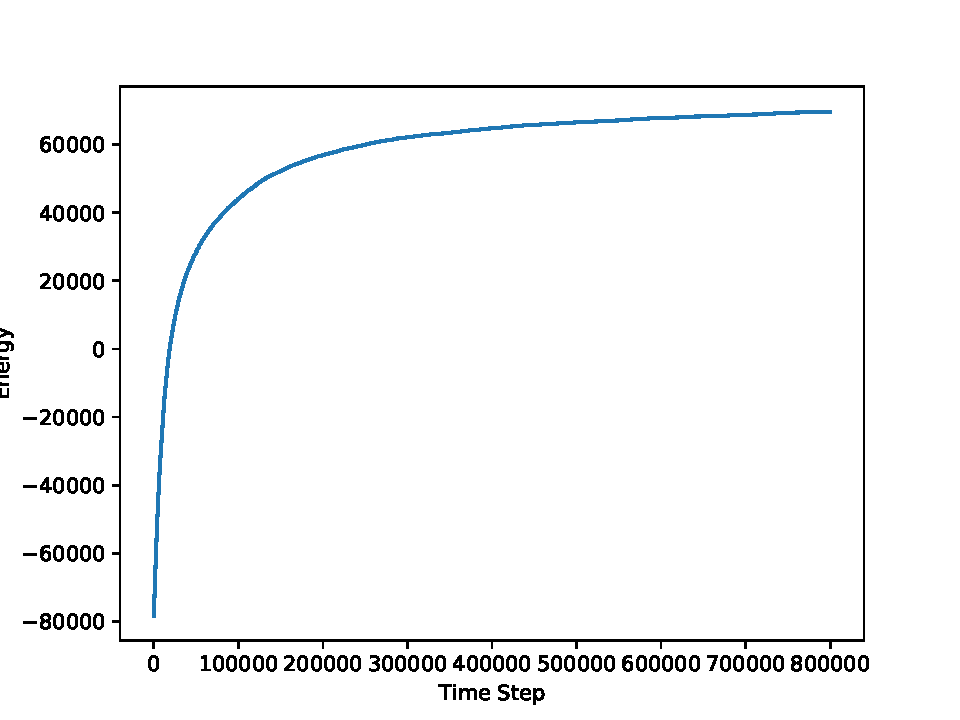
\includegraphics[scale=0.4]{g_e_0.pdf}
  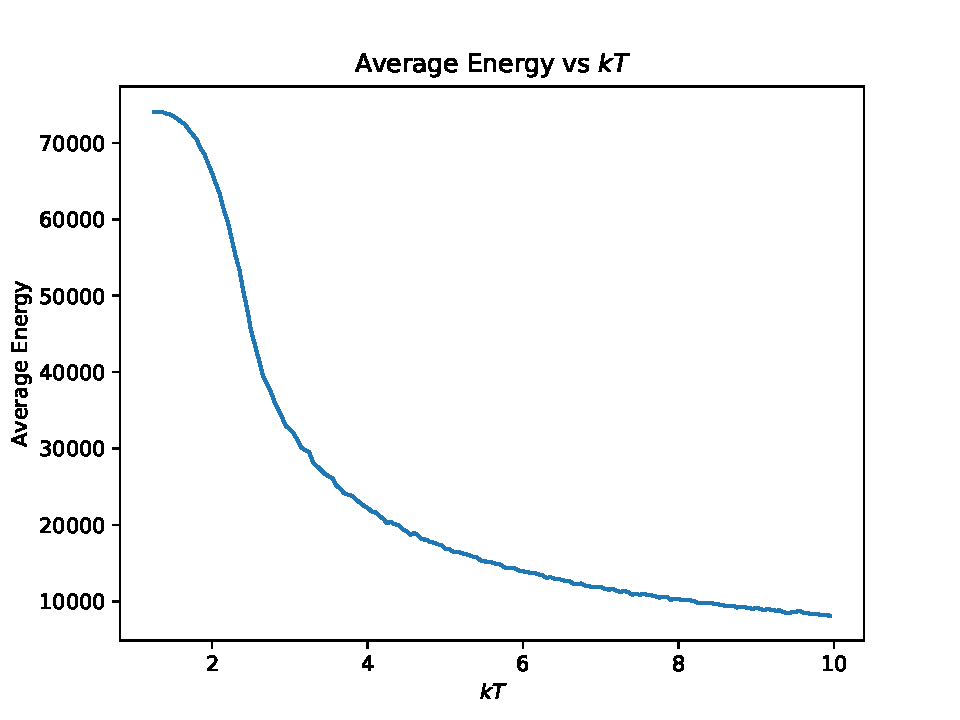
\includegraphics[scale=0.4]{g_avg_energy.pdf}
  \caption{\textit{(right)} plot of average energy vs $kt$.
    note an inflection at $\approx$ $kt = 2.5$, which is evidence of a
    phase transition.}
\end{figure}
\begin{figure}[H]
  \caption{\textit{(left)} Plot for average equilibrium magnitzation vs temperature.
  Note after a value of $kT \approx 2.5$ it begins to equilbriate.}
  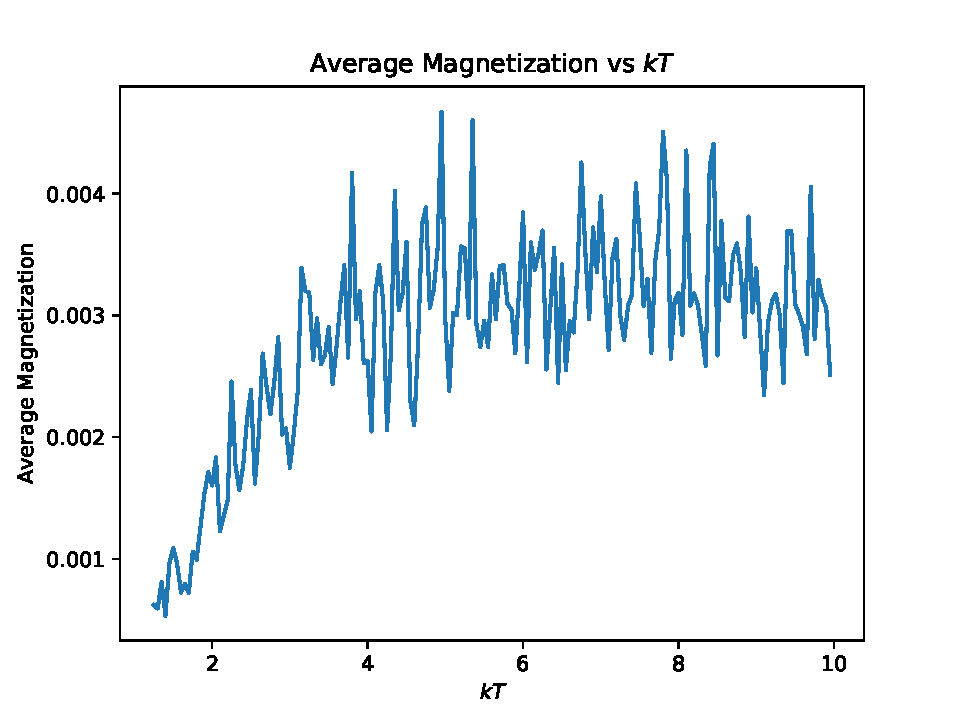
\includegraphics[scale=0.4]{g_mags.pdf}
  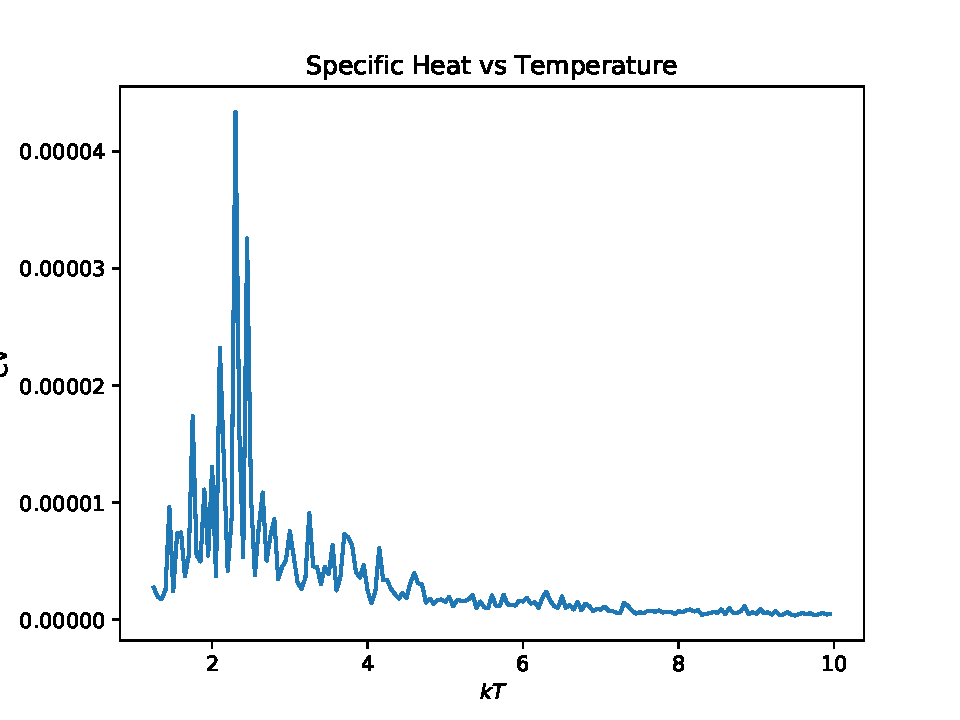
\includegraphics[scale=0.4]{g_cv.pdf}
  \caption{\textit{(right)} Plot for specific heat vs temperature. Note a peak at
  $kT \approx 2.5$, also indicating a phase transition.}
\end{figure}
\subsection*{All-adjacent}
\begin{figure}[H]
  \caption{\textit{(left)} Plot of Energy vs Time for $kT = 1$}
  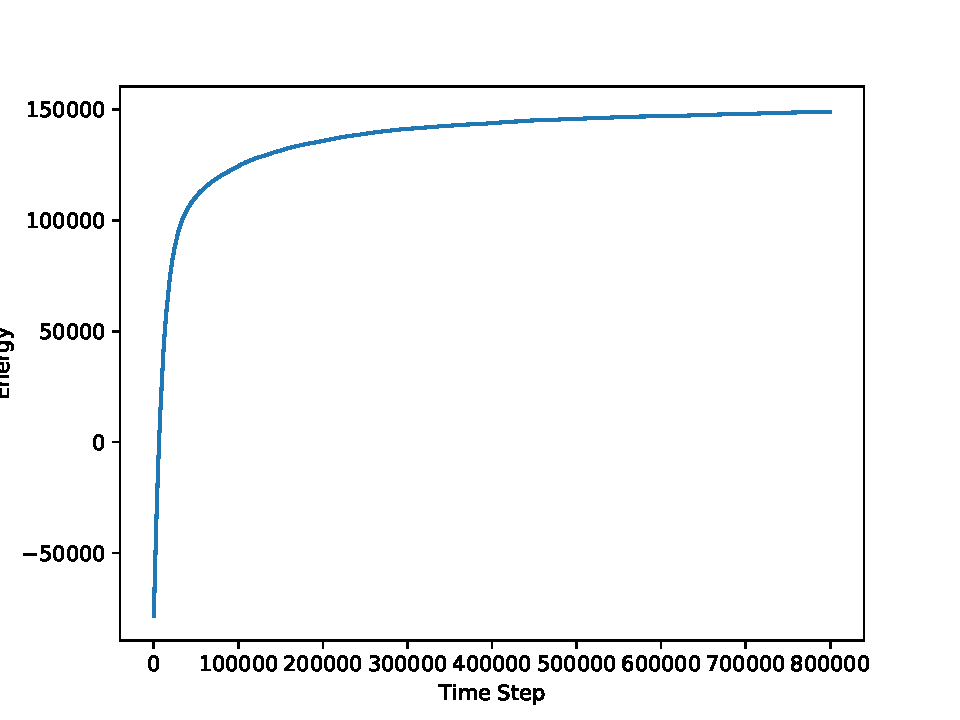
\includegraphics[scale=0.35]{a_e_0.pdf}
  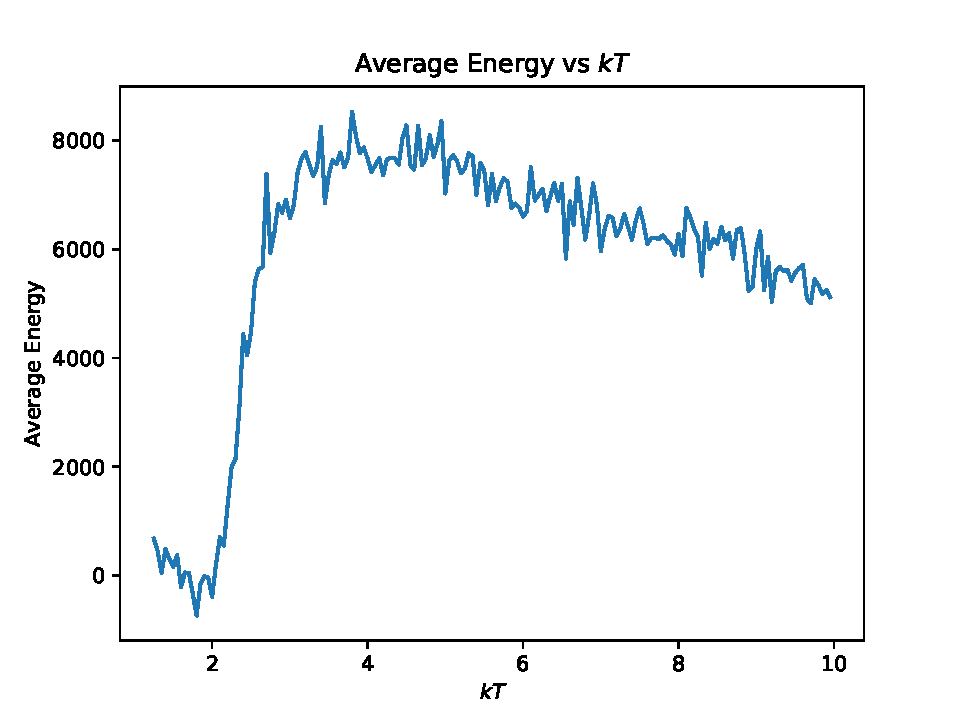
\includegraphics[scale=0.35]{a_avg_energy.pdf}
  \caption{\textit{(right)} plot of average energy vs $kt$.
    note an inflection at $\approx$ $kt = 2.2$, which is evidence of a
    phase transition.}
\end{figure}
\begin{figure}[H]
  \caption{\textit{(left)} Plot for average equilibrium magnitzation vs temperature.
  Note after a value of $kT \approx 2.2$ it begins to equilbriate.}
  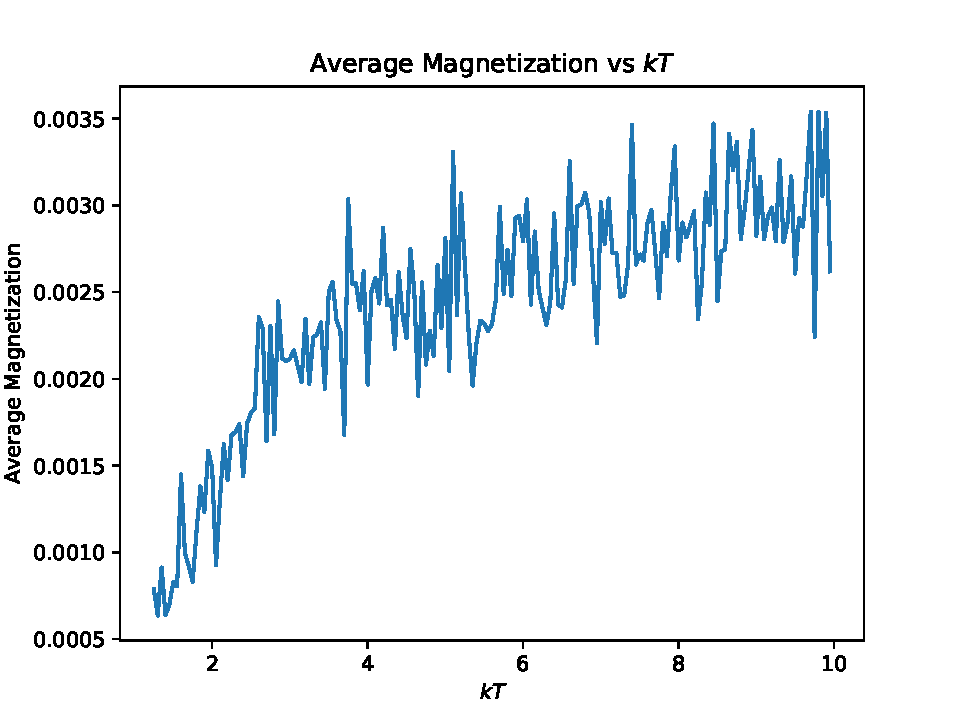
\includegraphics[scale=0.35]{a_mags.pdf}
  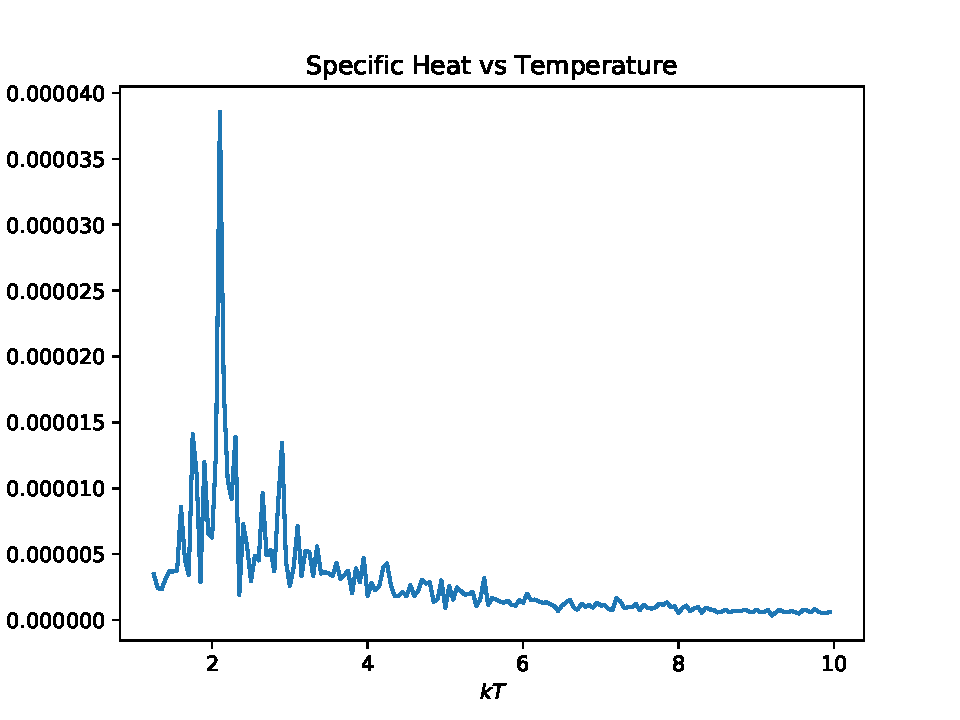
\includegraphics[scale=0.35]{a_cv.pdf}
  \caption{\textit{(right)} Plot for specific heat vs temperature. Note a peak at
  $kT \approx 2.2$, also indicating a phase transition.}
\end{figure}
\subsection*{Diag-adjacent}
\begin{figure}[H]
  \caption{\textit{(left)} Plot of Energy vs Time for $kT = 1$}
  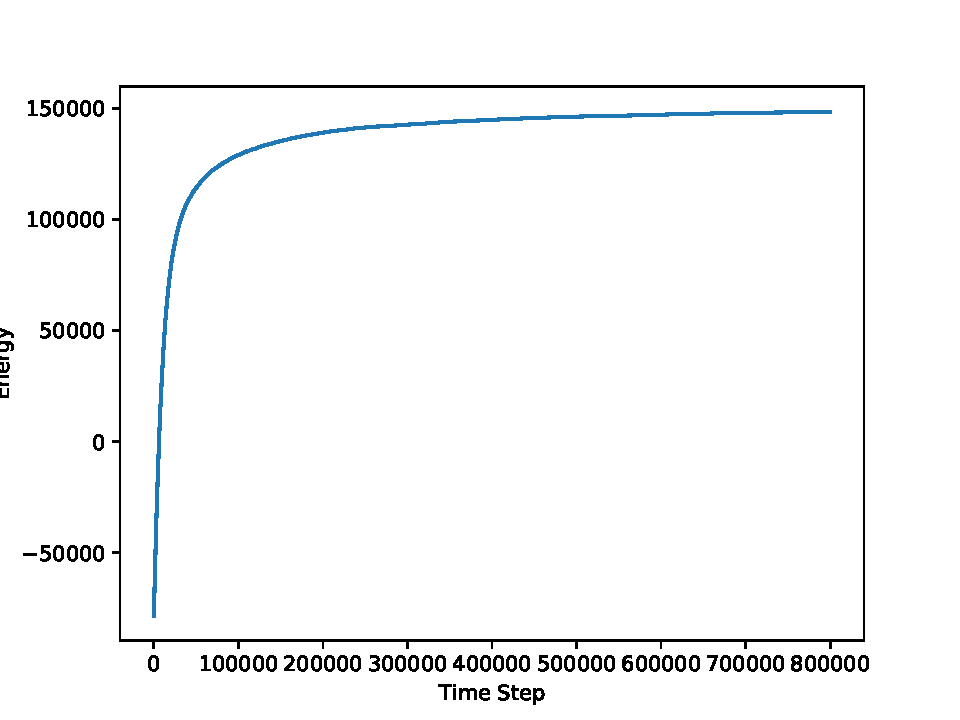
\includegraphics[scale=0.35]{d_e_0.pdf}
  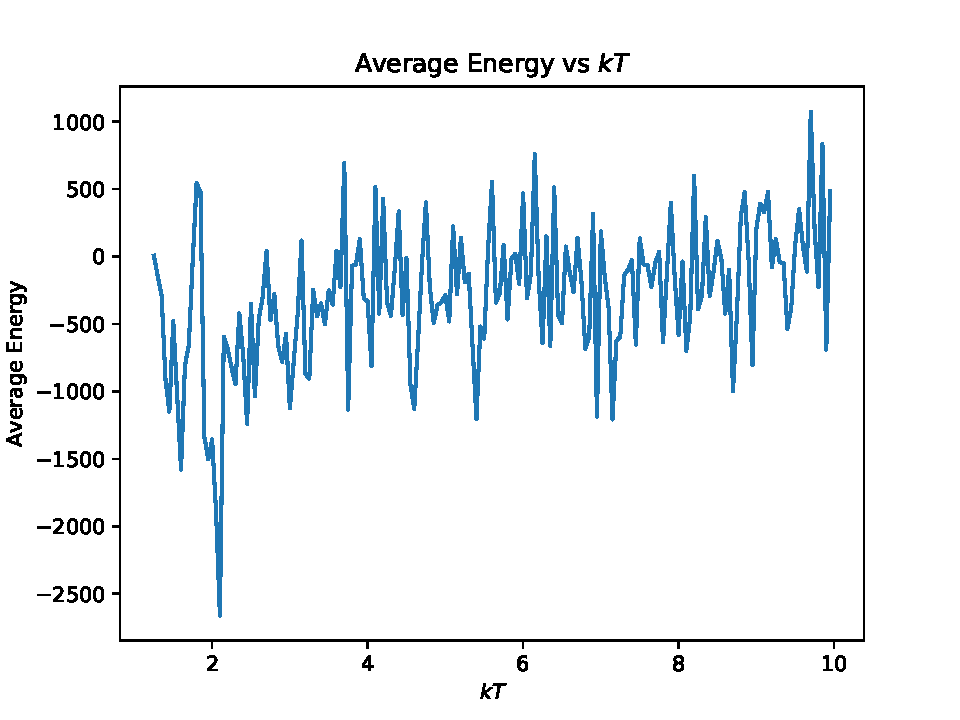
\includegraphics[scale=0.35]{d_avg_energy.pdf}
  \caption{\textit{(right)} plot of average energy vs $kt$.
    This graph is very noisy and no inflection point seems immediately discernable.}
\end{figure}
\begin{figure}[H]
  \caption{\textit{(left)} Plot for average equilibrium magnitzation vs temperature.
  Due to the noise this graph is hard to determine a phase transition temperature}
  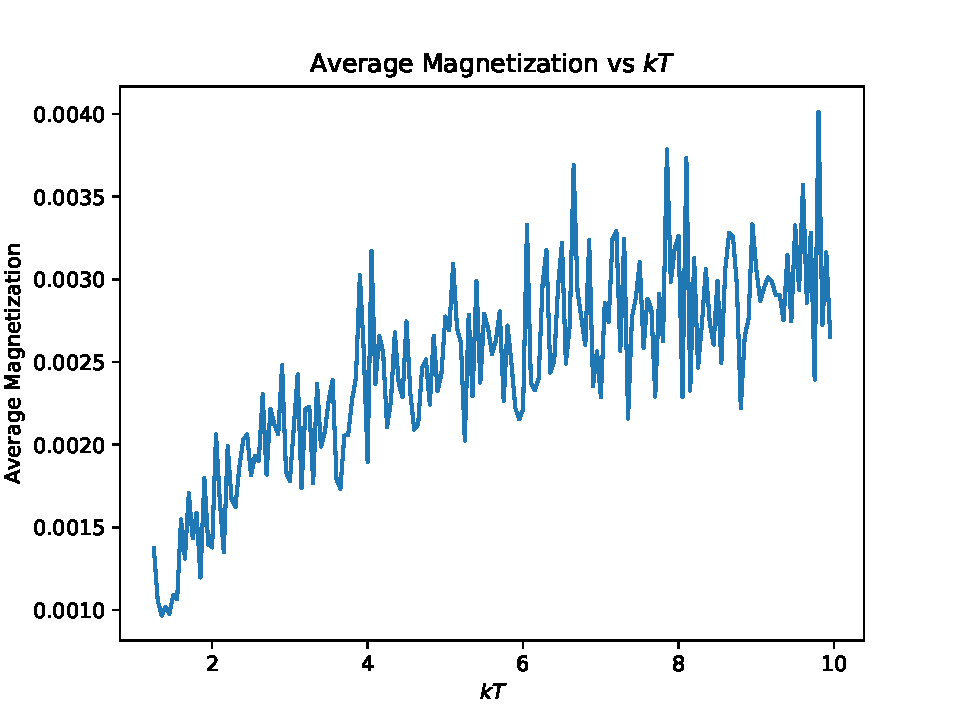
\includegraphics[scale=0.35]{d_mags.pdf}
  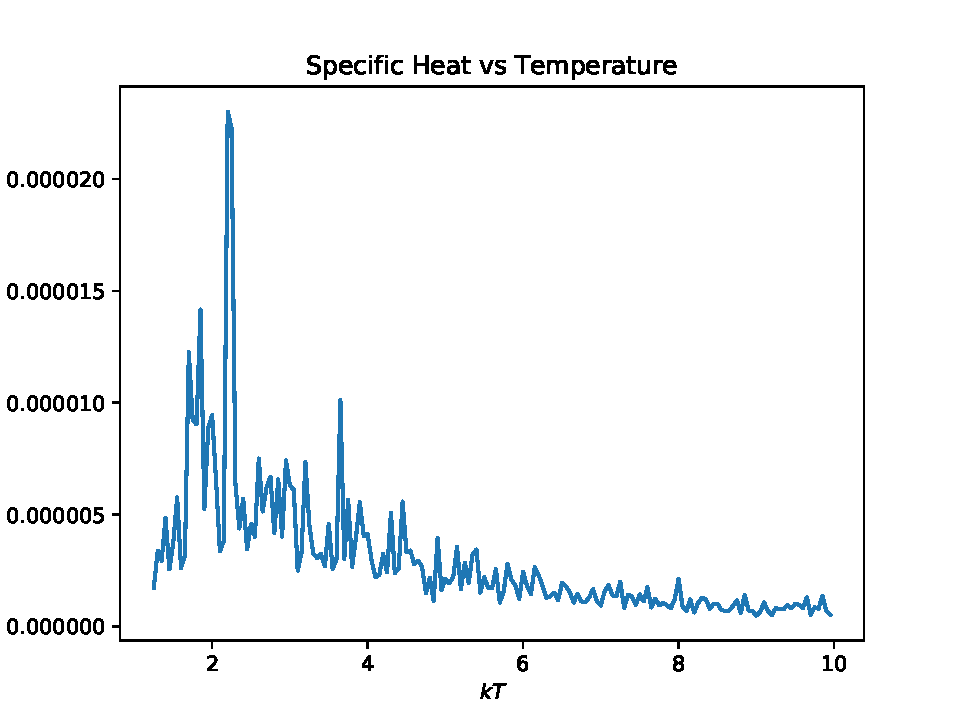
\includegraphics[scale=0.35]{d_cv.pdf}
  \caption{\textit{(right)} Plot for specific heat vs temperature. Note peaks at
  $kT \approx 1.8 $ and $kt \approx 2.1$}
\end{figure}
\section*{V. Analysis}
\indent \indent 
\section*{VI. Conclusion}
\end{document}
